%!TEX root = ../main.tex
\section{Umgehungsmöglichkeiten}
  \subsection{Ausweichen zu Alternativen}
    \begin{frame}<beamer>{Ausweichen zu Alternativen}
      \begin{itemize}
        \item Briefverkehr
        \item Apps für SMS versandt. (Whatsapp)
        \item alternative Emailprovider welche nicht überwacht werden.
        \item kritische Datenmenge: Für ein aussagekräftiges Profil müssen viel Daten gesammelt werden
        

      \end{itemize}
    \end{frame}
      \subsection{VPN,Proxy,TOR}
    \begin{frame}<beamer>{VPN,Proxy,TOR}
      \begin{itemize}
        \item VPN - Virtual Private Network 
        \item Webproxy
               \begin{itemize}
         \item Computer verbindet sich über das Internet zu einem Server und surft über diesem weiter
         \item Die Vorratsdatenspeicherung würde nur die Adresse des Webproxys speichern.
  
      \end{itemize}
      \end{itemize}
    \end{frame}
        \begin{frame}<beamer>{TOR}
      \begin{itemize}
        \item TOR ist ein Netzwerk zu Anonymisierung von Verbindungsdaten
        \item Verwendung für Webbrowsing, Instance Messaging IRC,SSH,Email
        \item TOR basiert auf dem Prinzip des Onion-Routings
        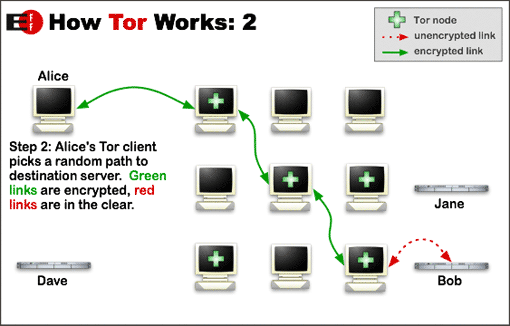
\includegraphics[height=0.7\textheight]{sections/img/tor_server_prinzip.png}
   
      \end{itemize}
    \end{frame}






